%
% Modified by Sameer Vijay
% Last Change: Wed Jul 27 2005 13:00 CEST
%
%%%%%%%%%%%%%%%%%%%%%%%%%%%%%%%%%%%%%%%%%%%%%%%%%%%%%%%%%%%%%%%%%%%%%%%%
%
% Sample Notre Dame Thesis/Dissertation
% Using Donald Peterson's ndthesis classfile
%
% Written by Jeff Squyres and Don Peterson
%
% Provided by the Information Technology Committee of
%   the Graduate Student Union
%   http://www.gsu.nd.edu/
%
% Nothing in this document is serious except the format.  :-)
%
% If you have any suggestions, comments, questions, please send e-mail
% to: ndthesis@gsu.nd.edu
%
%%%%%%%%%%%%%%%%%%%%%%%%%%%%%%%%%%%%%%%%%%%%%%%%%%%%%%%%%%%%%%%%%%%%%%%%

%
% Chapter 4
%

\chapter{MUON VETO DEVELOPMENT}
\label{chap:muVeto}
\begin{comment}
Explain some cosmic ray basics - only the stuff relevant to our detector (1 muon per square foot per second and MIP -> landau energy distribution).
Discuss materials available for veto and basic design decision of WLS
\end{comment}

\subsection{Testing with 26Mg}
\begin{comment}
Show results from first run and look at timing - hey it's all right!
Look at background - will need to improve
\end{comment}

\GeTargets cross-sections are predicted to be 300 mb, much lower than previous cross-sections measured with the neutron wall.  \Mg{26} has a cross-section of ?? mb and its differential cross-section (right word?) has been well measured by \cite{Bohne_Mg}.  Since its level structure is similar to \GeTargets in that is has a low-lying 0+ first excited state, \Mg{26}(\He{3},n) serves as an excellent system to test the neutron wall.

% figure: 26Mg level scheme (along with Ge level scheme?)

The TOF spectrum at the forwardmost angle is shown in Figure ??.  The neutron peak has a width of 1.2 ns and is clearly visible against the background.  Figure ?? shows the agreement of the extracted cross-section to previously measured data.

% figure: Bar A TOF spectrum

% figure: 26Mg cross-section compared to old data

The concerning thing about this data is that the neutron peaks at angles with low cross-sections do not stand significantly above the random background.  This has serious implications for the \GeTargets experiment, where the cross-section is suspected to be even lower.  Current data on two-proton transfer typically has errors no worse than 20\%; to achieve such errors it is necessary to either reduce the background or increase the beam current.  Increasing the beam current substantially was not feasable because of ion source limitations.  The background comes primarily from low-energy $\gamma$ radiation from the cement in the room and from muons produced by cosmic rays.  The next chapter discusses the construction of a cosmic-ray veto.

% introduction to cosmic rays
Sea-level radiation due to cosmic rays consists primarily of muons created in the upper atmosphere.  The energy distribution of muons incident on the neutron detector peaks at 100 GeV/C \cite{PDG}, so that most of the muons traveling through the detector are Minimum Ionizing Particles (MIP's).  This means that their energy loss is proportional to their path length in that material.  Muons at these energies deposit 1 MeV/cm2/g \cite{PDG}.  The detector consists of plastic with a density of ??, so the muons can deposit less than 0.5 MeV to 80 MeV depending on their path through the plastic.  It is possible to discard events that are more energetic than the highest-energy neutron, but most events deposit less energy and, if they arrive in the time window of interest, are indistinguishable from a neutron event.  The rate of such muons is low; one muon per square foot per second.  Of these, only a fraction arrives in the time window of interest, 20/400.  With a high flux of event neutrons, this background would pose little problem.  But the 76Ge(3He,n) cross section is predicted to be on order of ?? mb/sr.  Without vetoing the cosmic rays, the signal will be outnumbered ?? to 1, greatly increasing the uncertainty in the absolute cross-section. 

Impractical solutions to muon background abound.  One may wish to go deep underground, giving the muons more time to decay and thus reducing their flux.  This is not feasible because the ion source and accelerator infrastructure necessary to do this experiment do not currently exist in any underground laboratory.  Another solution would be to remake the neutron detector, using a material that can distinguish between neutron and muon interactions.  Such scintillators exist [CITE!], but are typically toxic, flammable, liquids.  A large-angle detector made of such scintillator would be doubly helpful because these scintillators can distinguish between neutron and $\gamma$ radiation, as well, which would reduce another significant source of background signal.  Working with such difficult material, however, was beyond the scope of this project; the goal was to make a manageable change to the existing detector to reduce muon background. 

A practical solution to the muon background is to make a veto shield that registers the likely presence of a muon.  The now-identified muon event can then be discarded.  Distinguishing between muons and non-charged particle interactions using additional scintillator material is possible because of the difference in likelihood of interaction.  
\begin{figure}[hp]
\centering
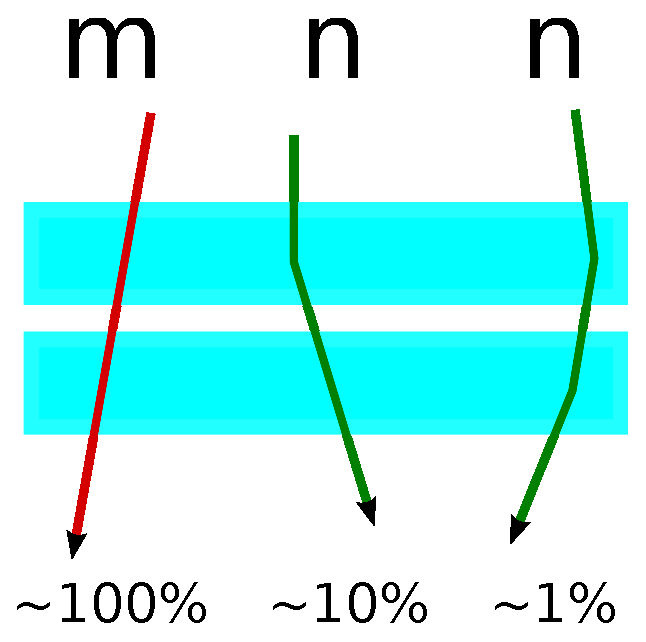
\includegraphics[width=1.0\textwidth]{figures/simpleVeto.eps}
\label{fig:simpleVeto}
\caption{The charged muon has a nearly 100\% chance of leaving a detectable signal in both scintillators, while the neutron, lacking charge, is much less likely to interact in even one of the scintillators.  The likelihood of detecting a neutron interaction depends on both the thickness of the scintillator and the threshold of the detector; for a 5 cm thick scintillator with a threshold at approximately the Th edge, the likelihood of detecting a 20 MeV neutron is about 10\%.}
\end{figure}
While the charged muon will almost certainly leave a detectable signal in both scintillators, the neutron is highly unlikely to do the same.  The bars of the neutron detector are 5 cm thick; the chance of detecting a 20 MeV neutron when the detection threshold is at approximately the Th edge is 10\%.  The chance of one neutron interacting in two bars, then, is only 1\%.  If the muon veto is made of a thinner bar of scintillator, the probability of a detectable neutron interaction in both drops further.  By placing a thin ($\sim$1 cm) scintillator over the neutron detector bar, it is possible to identify muons to an accuracy of at least 0.99\%.  Note that such a veto does not identify $\gamma$ radiation because it has an efficiency similar to neutrons.

\section{Light Collection with WLS}
\begin{comment}
Describe light collection with WLS
Explain why we loop the WLS and collect light from both ends
Discuss the light limitations of light guides (Liouville) and ways to increase light collection with WLS (more!)
Describe fragility of WLS, how some efforts make custom plastic clamps to make it robust, how this doesn't work for you so you made a break and attached a cable.  Discuss signal loss.
\end{comment}
The scintillator bars of the neutron detector are outfitted with two PMT's, each coupled to its end via a non-scintillating light guide.  Having two PMT's is essential both for good timing information and also to lessen the position sensitivity of the signal that is inevitable with such a large detector.  Instrumenting the veto scintillator in this way was not feasible.  Fitting a top and bottom PMT to each veto bar would require 32 PMT's and lightguides, along with independent power supplies for each.  Instead, Wavelength-shifting fiber (WLS) was chosen to collect the light.

WLS collects light by absorbing broad-spectrum radiation and re-emitting that light in the green.  It is possible to coat the fiber with material with an index of refraction that guarantees total internal reflection for green light, and so the light bounces in the fiber until it reaches a detector.  Because light can travel in two directions in the fiber, looping the fiber so that both ends terminate in a detector collects the most light.  Sometimes this is not possible and the ends of the WLS are silvered, but this is an expensive process and does not recover all the light.  WLS largely eliminates position sensitivity because it can be arranged on the detector so that no part is distant from the collecting fiber [cite??]; laying the fiber in a loop on the detector often means that only one PMT is required.

The disadvantage to WLS is light intensity [cite??] and fragility.  Sufficient light intensity to boost the signal above the noise is a serious concern, and is often overcome by using many WLS strands to collect light [cite NASA thing, show picture?].  The fragility of the WLS is more difficult to remedy.  Maximum light collection dictates taking the fiber on the detector directly to the PMT, which should be as close to the plastic as possible to minimize the length of this fiber run.  Because two bars needed to share a PMT, some plastic was 2 m away from its PMT.  At this length, enclosing the end of the detector, the WLS fiber, and the PMT in an immovable cast was not practical.  And with free-floating ends, the fiber quickly degraded and snapped, even with careful handling.  Dismayed at the possibility of making detectors and mounting them to the neutron detector only to have the fragile fibers carrying their signal snap, leaving us with no way to access their signals, the design was dramatically altered.  The WLS was cleanly severed at the end of the plastic and a robust cable was made to attach to the WLS.  Certainly severing the WLS causes significant light loss, but with the benefit of durability.  

\section{Paddle Design}
\begin{comment}
Schematics
Tolerances
Making sure the transmit cable lines up with the paddle WLS fibers!  Dowels.  Tolerance doesn't actually need to be that good
connecting cable with PMT
cable design - hosing for protection
\end{comment}

There are three constraints for the paddle-cable interface.  The diameter of the cable must be larger than the diameter of the WLS so that small misalignments do not greatly impact light collection.  The center of the cable must be aligned to the center of the WLS.  Lastly, the cable must be robust.

\begin{figure}[ht]
\centering
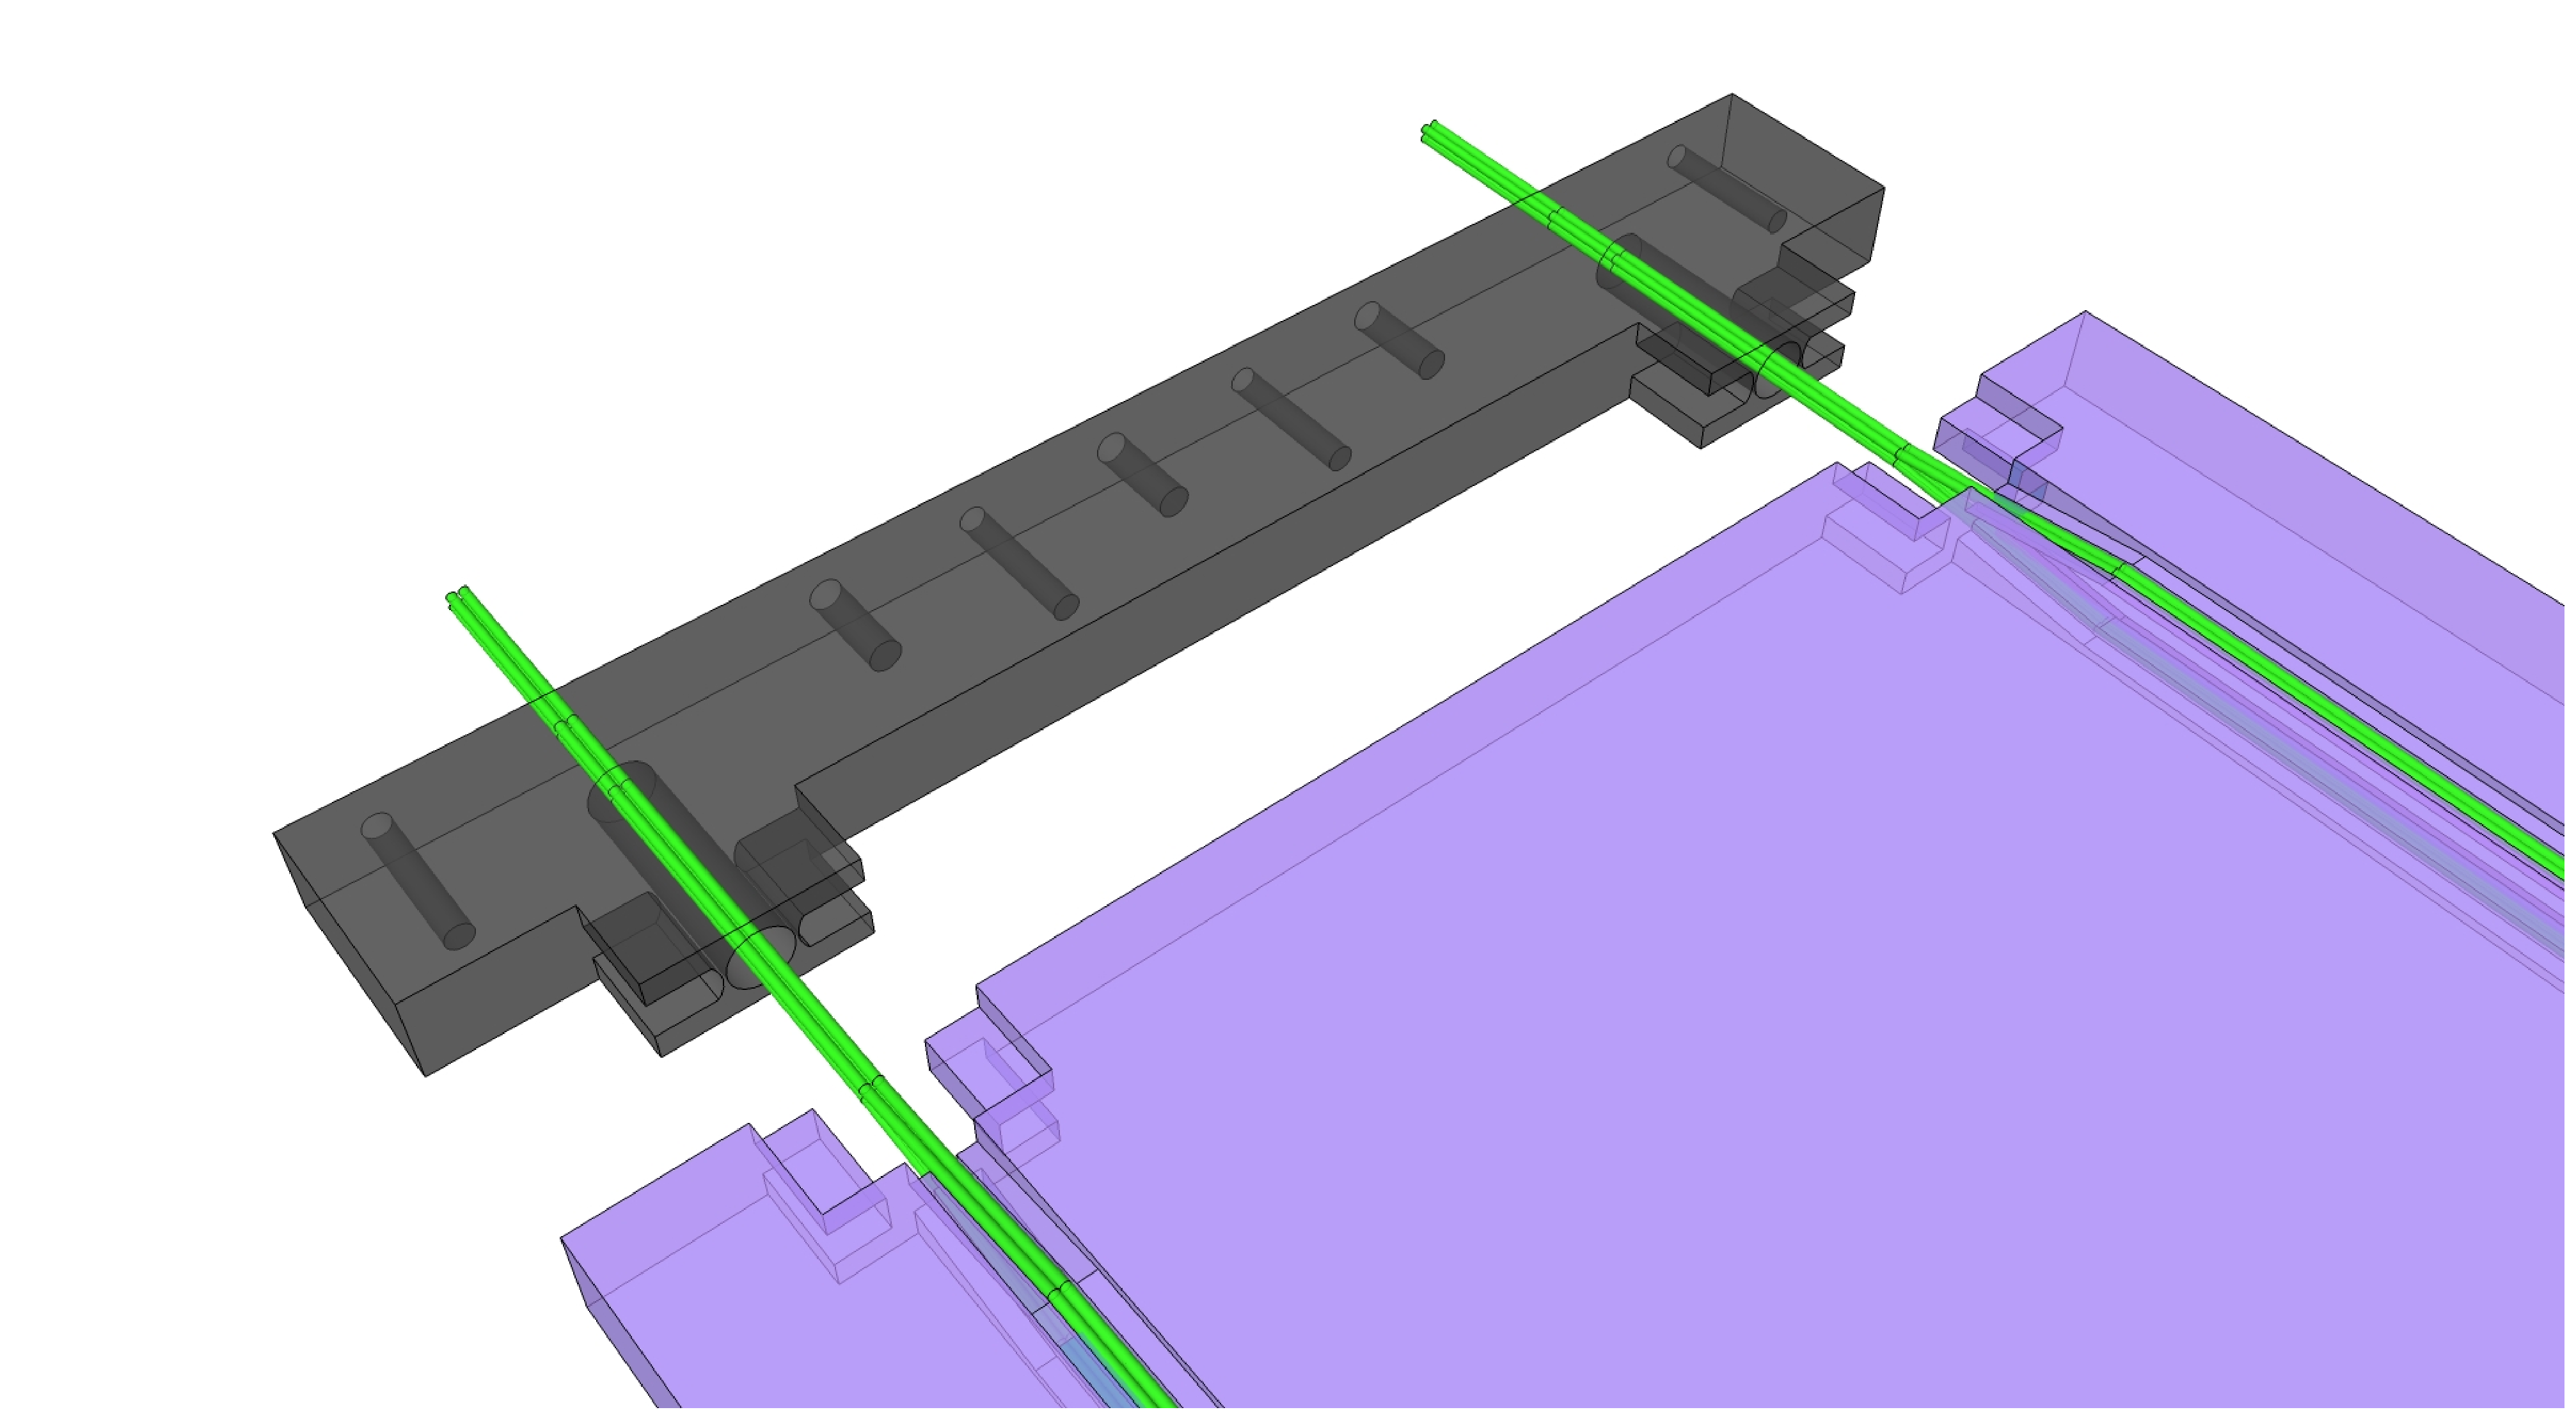
\includegraphics[width=1.0\textwidth]{figures/veto_assembly.eps}
\label{fig:paddleAssembly}
\caption{The endcap will be glued to the scintillator after it is slid into place.}
\end{figure}

% talk about the diameter of the WLS and the alignment
The diameter of the WLS on the paddle is ?? mm.  The mating cable has a diameter of ?? mm and is optimized for transmission rather than collection.  Its larger diameter enables it to completely overlap the WLS as long as the centers are aligned to within 0.1 mm.  To ensure this level of alignment, tight-fitting dowels align the region of the cables containing the fiber cluster.  This is particularly important because the connectors are machined from plastic and often are not perfectly square - some connectors bow as much as 20 mils from normal.  The only regions that must be carefully aligned, however, are the fiber clusters, and the dowels constrain these regions to less than ?? mils, ensuring an alignment of ?? mm.  

% talk about the cable housing
Another design constraint is that the support for the cable fiber must resist bending that would damage the fiber but also be flexible enough to route to the PMT.  Stiff, rubber tubing (durometer rating = ??) coupled to a hose barb housing the fibers limits the bending to a safe radius.



\section{Paddle Performance}
\subsection{tests on intrinsic efficiency}
\begin{comment}
Show signal from detector
Talk about first tests?  Can talk about sensitivity to geometric alignment of trigger paddles ...
Maybe mention this and then be like, ``this is why we decided to look at the efficiency this other way that was less sensitive''
\end{comment}
In principle, testing the intrinsic efficiency of the paddles is simple.  Requiring a coincidence with several paddles whose arrangement forces the path of the muons to intersect the volume of the veto paddle is successful at 

1. restricting the counts to muons and
2. ensuring 100\% geometric efficiency

In practice, arranging the available scintillator to force muons through the test volume was difficult because the available scintillator was instrumented with bulky lightguides and could not be laid directly on the test volume.

Using our cosmic ray simulation program, we determined an arrangement that maximized geometrical efficiency.  This arrangement, however, was extremely sensitive to placement; measured efficiency of the same bar could change from 98\% to 75\% with a displacement of a few centimeters.

For this reason, testing efficiency of the bars was done in a different way.  [Oh was it now?].

\subsection{On-Detector Efficiency}
\begin{comment}
Initial efficiency - would be nice to show this data
Describe different cosmics that hit the neutron bar but miss the veto - argh!
Discuss changes made to mounting to improve coverage - show new data (cosmics)
\end{comment}
The veto paddles were initially mounted 2 cm from the neutron detectors, not because of calculated optimization but because we wanted to mount the veto without removing (and potentially damaging) the heavy neutron detectors.

Running a test with 26Mg(3He,n) showed good cosmic rejection in the two innermost bars of each four-bar unit and worse rejection in the outer two bars by about 20\%, corresponding to double the cosmic background.  This is sensible, as the outer bars act as additional veto for the inner bars, while the outer bars enjoy no such additional information.  Wishing to improve the background rejection for the outer bars, we wrote code that simulated the cosmic background to understand best placement for the veto material.

Simulations agreed well with experiment [this is like very expandable, dear].  Material needed to be added to the sides of the outermost neutron detectors, and significant gains in veto efficiency could be had by moving the veto material as close as possible to their neutron detector.  Additionally, efficiency improves when the neutron detectors (and the veto material in front of them) are moved as close together as possible.  All these changes resulted in improved, nearly uniform veto efficiency across the detector.

\begin{figure}[ht]
\centering
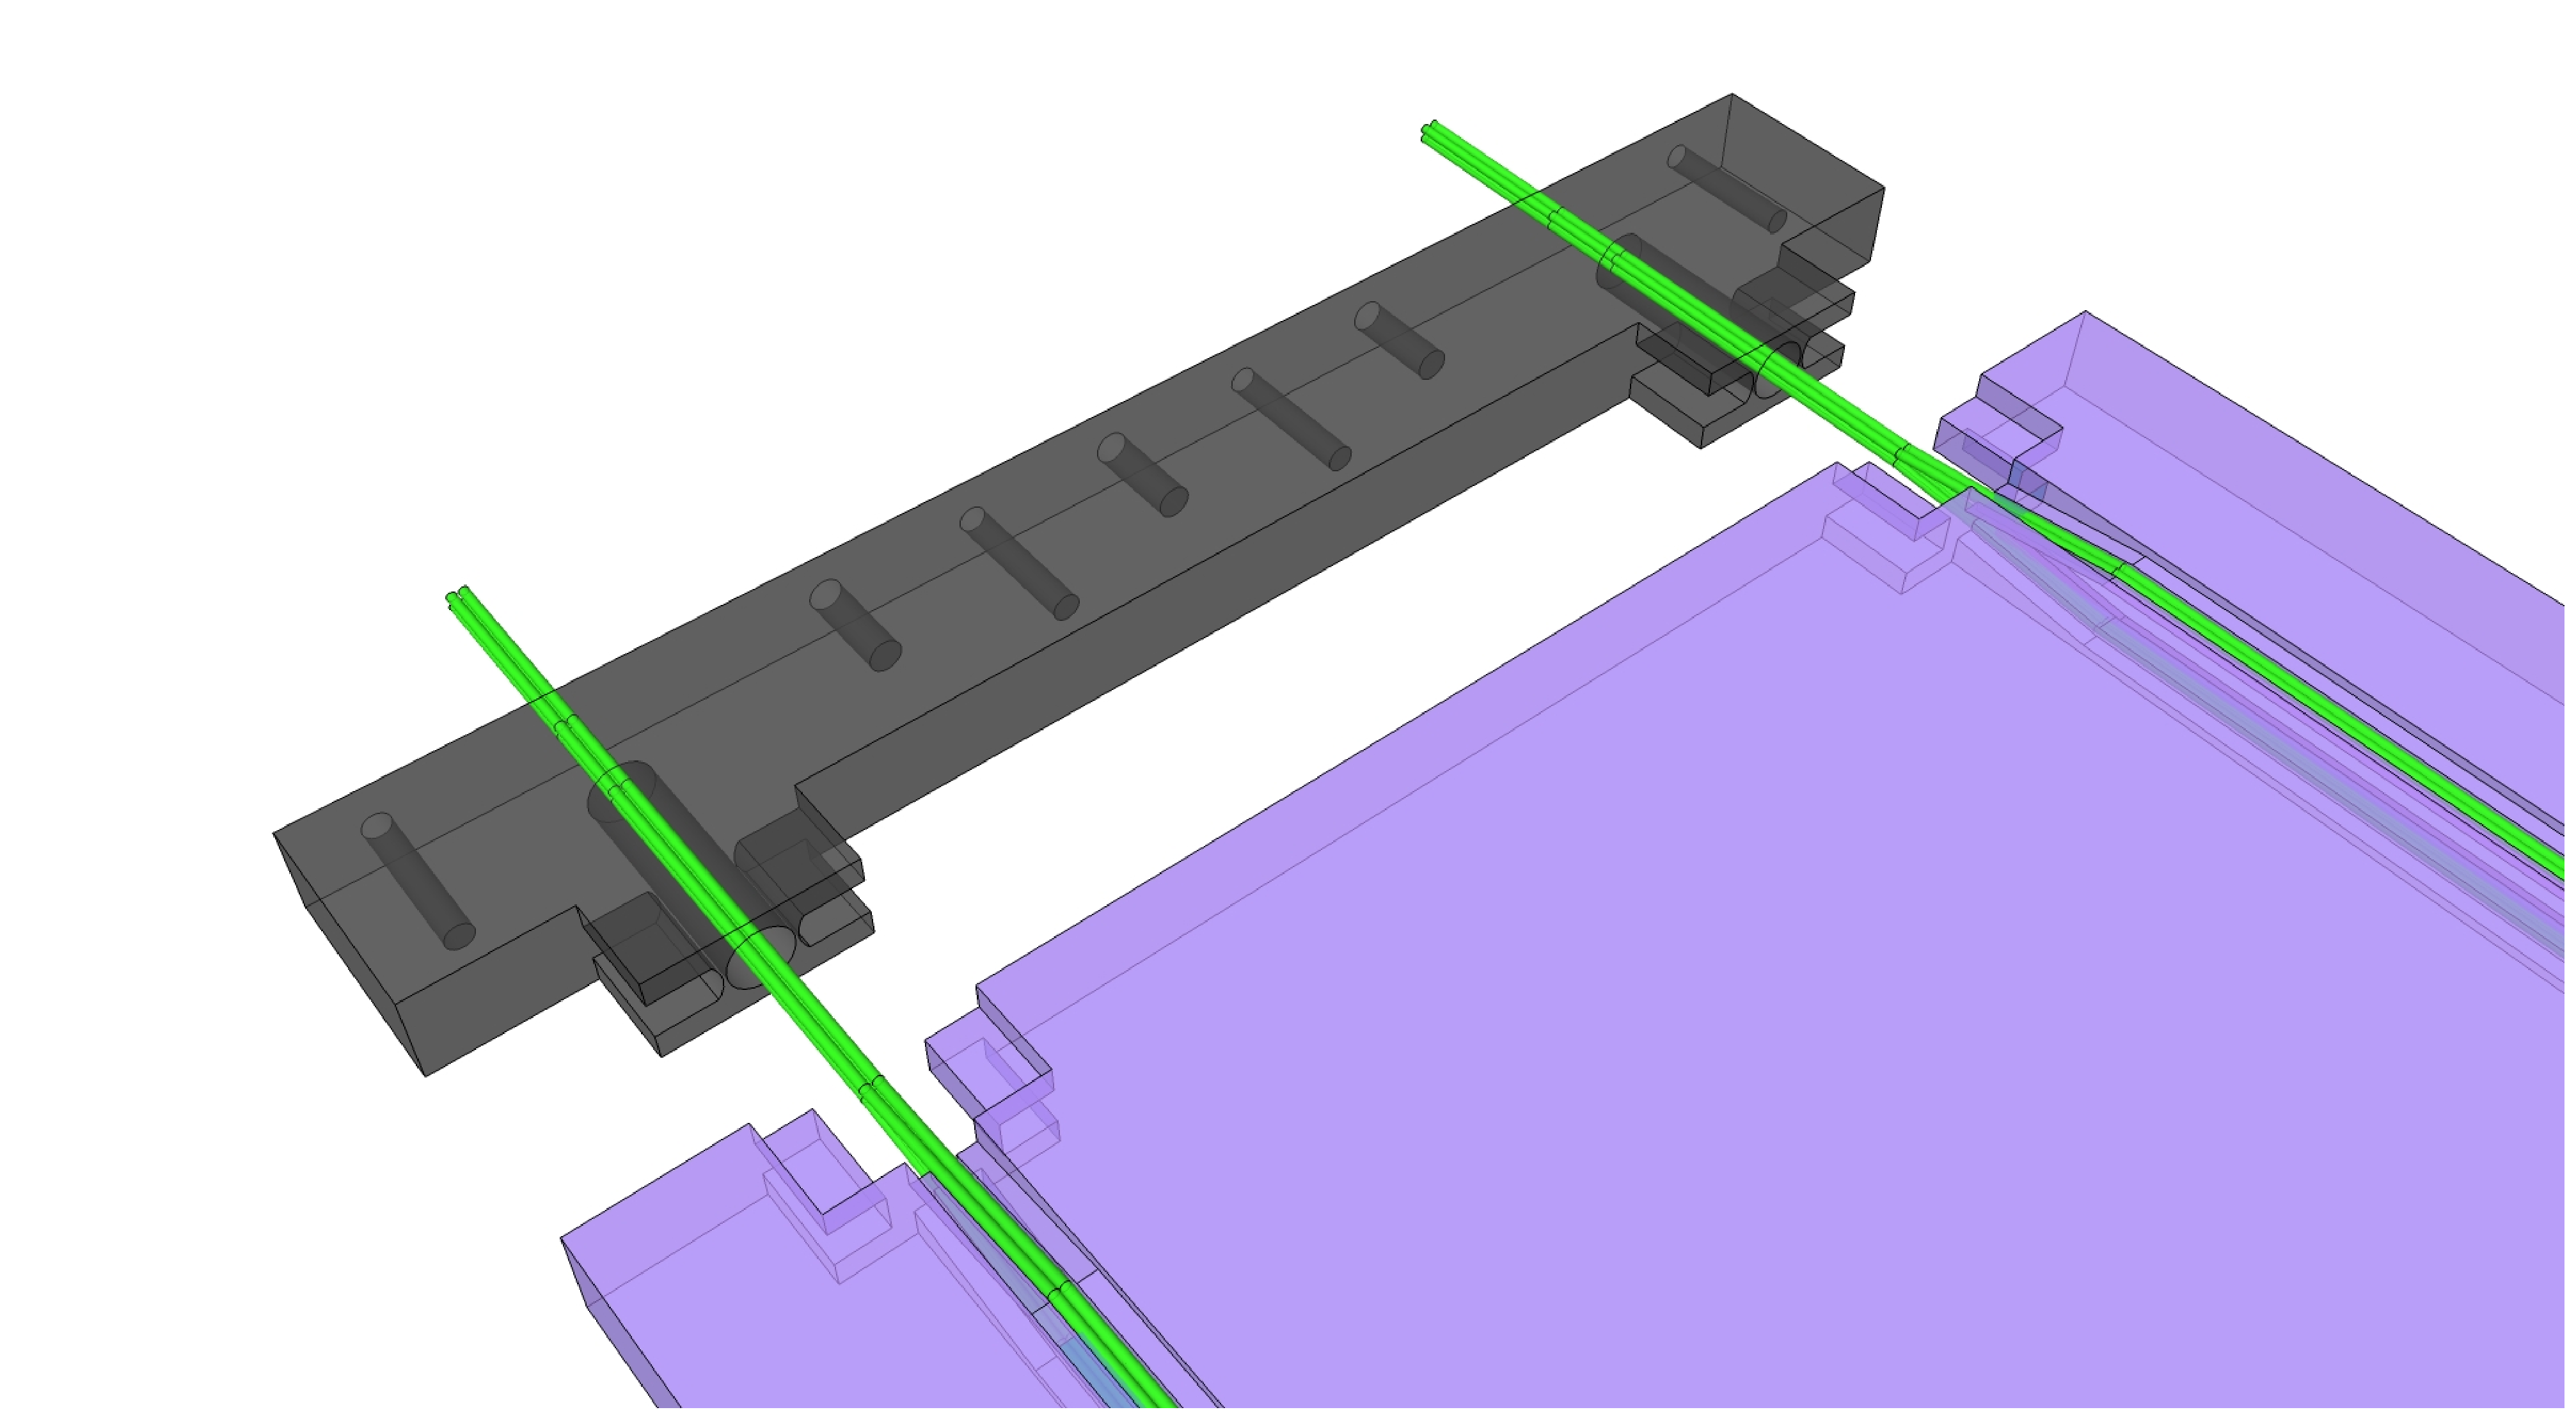
\includegraphics[width=1.0\textwidth]{figures/veto_assembly.eps}
\label{fig:compareEfficiency}
\caption{Efficiency before side veto material and compression and after.}
\end{figure}

\section{Electronics}
\begin{comment}
Originally wanted to use timing information but there weren't enough channels
Bit Register - give example
discuss random rate and estimate how often you'll fire during a real event and also how often one bar will fire with something real, vetoing a real event
LeCroy 4532 - MALU - majority logic unit ``The status of up to 32 inputs can be monitored and recorded by issuing a strobe.  Since the inputs are edge-triggered, the strobe may be a gate of arbitrary duration.  Then any inputs which are on during any portion of the gate are recorded and stored in a pattern register.'' (from the manual).
\end{comment}
As mentioned above in section ??, testing efficiency was done using a timing spectrum.  With 24 bars, however, we did not have sufficient TDC channels to record timing information for the full veto.  One readily available module was a Bit Register.  A bit register has a certain number of inputs, typically 16.  The bit register also has a gate.  Each input corresponds to a bit in an integer with 16 bits.  When the gate is high, the bit register records the number built by the voltages on its inputs.  This number, then, shows which detectors fired when the gate was high - exactly the information we need!

Recording the integer generated by the bit register instead of the time of the signal relative to the beam bunch is a loss of information.  The gate provided to the bit register is a copy of the event trigger and is 200 ns wide.  The signals sent to the bit register inputs that overlap the gate signal will increment the bit pattern and are 20 ns wide.  The LeCroy 4532 applies an edge-trigger to the inputs, so the maximum time difference between an event in the neutron detector and an event in the veto that will still be recorded in the bit pattern is the width of the gate signal, 200 ns.  This compares unfavorably to the timing spectrum, where even with a leading edge discriminator, the timing peak has a width of less than 5 ns.

The concern, of course, is accidental vetoing.  We work hard to get our neutron events and do not wish to throw them away because a background gamma left a signal in the veto within 10 ns of a real neutron signal in the neutron detector.  Accidental coincidences come from non-beam-related background radiation, both cosmic (not too frequent) and gamma (quite frequent at low energies).  Fortunately, the rate of this ``noise'' is not so high that using the bit register instead of a TDC increases the accidental veto rate by any significant amount.  The trigger rate of a typical veto paddle is 1000 Hz.  Certainly some of these events are true cosmic muons, but to obtain an upper bound we treat this as the noise rate.  The probability that a noise event will occur within the window allowed by the bit register is 

\begin{equation}
\frac{Rate}{Time Window} = \frac{1000 Hz}{200 ns} = 5\times10^{-8}.
\end{equation}
With a number of triggers of approximately 10??, the expected number of rejections based on unrelated background is a scant 20?? counts.

\section{Beam Tests}
\begin{comment}
What data should I show?  Old Mg vs. New Mg?  Or New Mg with no veto vs.  New Mg with veto?
show the vetoed spectrum - put a limit on how much real signal is rejected?
\end{comment}

\subsection{Rejected Signal}
\begin{comment}
Two causes for rejected signal
1. the bars are ganged together; could get a signal in one veto bar that does not mean there was a cosmic in its adjacent neutron detector
2. randoms

can place a limit on randoms, reals, and therefore good rejected signal
\end{comment}

% % uncomment the following lines,
% if using chapter-wise bibliography
%
% \bibliographystyle{ndnatbib}
% \bibliography{example}
